\section{Controlerkomponente VCM-Wrapper}
\subsection{Zusammenfassung}
Der VCM-Wrapper spiegelt der Eclipse-Plattform ein vollfunktionsf�higes Team-
Plugin vor, �ber das alle Repositoryoperationen durchgef�hrt werden. Intern
gibt die Komponente die Aktionen jedoch an andere Team-Plugins weiter. Vor und
nach jeder dieser Aktion wird die Kommunikations-Komponente konsultiert, um 
den Server bzw. andere Clients �ber Ver�nderungen am Repository zu 
informieren. Die VCM-Wrapper-Komponente kennt sowohl die Datei-Ebene und deren
Repositories als auch die Abstraktion auf Produktlinien/Komponenten/Varianten.
F�r beide Ebenen lassen sich atomare (z.B. checkin) und komplexe VCM-
Aktionen () ausf�hren. Die n�tigen Informationen �ber 
Repository-Positionen und Struktur bezieht der VCM-Wrapper �ber die Server-
Kommunikations-Komponente sowie das Architekturmodel.

%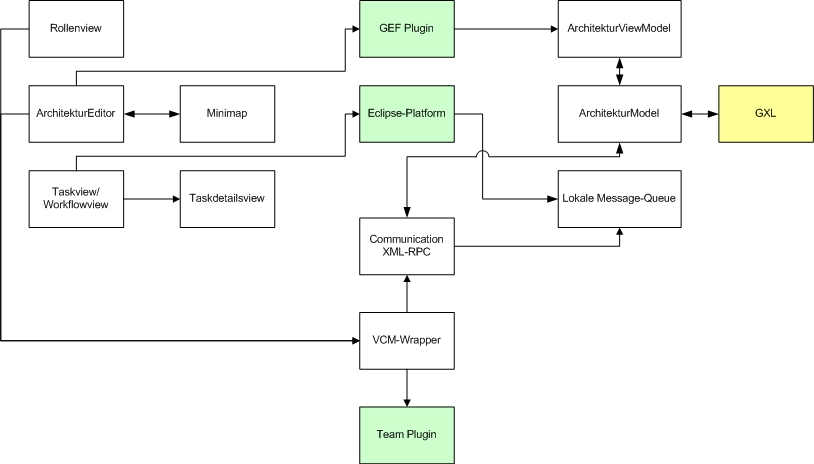
\includegraphics[width=15cm]{client.jpg}

\subsection{Manueller Import der Einstellungen}
Der Client meldet sich mit Benutzernamen und Passwort am Server an un
erh�lt vom Server eine spezifische Session-ID. Danach werden vom
Server alle Konfigurationsdaten geladen und diese automatisch in
Eclipse gespeichert. 
\par 
Durch diese Konfigurationsdaten kann Eclipse entscheiden welche
Repositories, zugeh�rige Rollen und Zugriffsrechte benutzt werden
m�ssen.
Dadurch k�nnen in Eclipse durch die erhaltenen Rollen und
Repository-Daten die vordefinierten Felder zum Zugriff auf
VCM-Repositories entsprechend gesetzt werden. Hierdurch wird eine
optimale Anbindung an bereits existierende Eclipse-Strukturen
geschaffen. 

\subsection{Automatischer Import der Einstellungen}
Falls der Benutzer das erste Mal Eclipse startet, d.h. noch keine
Konfigurationsdaten zu Rollen und Repositories vorliegen, findet ein
automatisches Login am Server statt, und seine Konfigurationsdaten
werden vom Server geladen und in Eclipsae gepeichert, wie im manuellen
Import n�her beschrieben.

\subsection{Automatischer Login bei wiederholtem Zugriff}
Beim ersten Login am Server wird von diesem eine eindeutige Session-ID
vergeben, die bei erneutem Zugriff auf den Server zur
Authentifizierung genutzt wird. Damit ist gemeint, dass dadurch das
erneute eingeben des Benutzernamens und des Passwort nicht notwendig
ist.\par
Falls der Server bemerkt, dass die selbe Session-ID zur
Authentifizierung von 2 verschiedenen Clients verwendet wird, wird
diese ung�ltig. Als folge dessen muss sich der Benutzer erneut mit
Benutzernamen und Passwort authentifizieren und erh�lt eine neue
Session-ID. Daher sollte beim Arbeiten eines Benutzers von verschieden
Client-Rechner unbedingt f�r jeden Arbeitsplatz eine eigene Session-ID
benutzt werden.

\subsection{Ablaufschritte beim Zugriff auf das Repository}

Die Ablaufschritte:\par

\begin{itemize}
    \item Lade Konfigurationsdaten vom Server (fetch)
    \item Extrahiere Rollenzuteilung, Repository-Daten
    \item Lokale Pr�fung auf vorhandenes Produkt, d.h. Produktdaten, Benutzerdaten (check)
    \item Pr�fungsergebnisse f�hren bei nicht vorhandenem Produkt zu
    �ffnendem Dialog und anschlie�ender Lade-Aktion (checkout) aus dem
    Repository
\end{itemize}\par

\section{M�gliche Wrapper-Aktionen}

Die sichtbaren Aktionen:\par

\bf Alle Benutzer:
\begin{itemize}
  \item check out: 
  \item update:
\end{itemize}

\bf Nur bestimmte Benutzer:

\begin{itemize}
  \item commit:
  \item import:
  \item delete:
  \item add:
\end{itemize}
